\documentclass[11pt]{article}
\usepackage[margin=1in]{geometry}
\usepackage{amsmath,amssymb,amsthm,mathtools}
\usepackage{booktabs}
\usepackage{enumitem}
\usepackage{hyperref}
\usepackage{tikz}
\usetikzlibrary{arrows.meta,calc,positioning,fit,shapes.geometric}

\newcommand{\State}{\ensuremath{\mathsf{State}}}
\newcommand{\View}{\ensuremath{\mathsf{View}}}
\newcommand{\Worldline}{\ensuremath{\mathsf{Worldline}}}
\newcommand{\Strand}{\ensuremath{\mathsf{Strand}}}
\newcommand{\Braid}{\ensuremath{\mathsf{Braid}}}
\newcommand{\Conflict}{\ensuremath{\mathsf{Conflict}}}
\newcommand{\Witness}{\ensuremath{\mathsf{Witness}}}
\newcommand{\Lower}{\ensuremath{\mathsf{Lower}}}
\newcommand{\Merge}{\ensuremath{\mathsf{Merge}}}
\newcommand{\Proj}{\ensuremath{\pi}}

\theoremstyle{definition}
\newtheorem{observation}{Observation}
\newtheorem{principle}{Principle}
\newtheorem{example}{Example}

\title{Merge Lifting Worked Examples\\[6pt]
\large From Ordinary Git Pain to Causal / Optic Merge\\[3pt]
\normalsize 2026-04-09}
\author{}
\date{}

\begin{document}
\maketitle

\section{Purpose}

This note turns the merge-geometry claims into concrete examples.

The structure is:
\begin{enumerate}[leftmargin=2em]
\item start with an ordinary merge problem,
\item show the lossy lowered surface,
\item lift the problem into richer causal nouns,
\item merge there,
\item lower back with witness,
\item classify the result as spurious conflict, genuine conflict, or governance
  conflict.
\end{enumerate}

\section{Example A: A Spurious Text Conflict}

\subsection{The ordinary file}

Suppose the public artifact is a one-line JSON file:

\begin{verbatim}
{"flags":{}}
\end{verbatim}

Branch A changes it to:

\begin{verbatim}
{"flags":{"admin":true}}
\end{verbatim}

Branch B changes it to:

\begin{verbatim}
{"flags":{"beta":true}}
\end{verbatim}

At the ordinary text surface, both branches touched the same line. A naive
line-based merge sees overlap and may conflict.

\subsection{What the richer state really is}

The richer causal state is not one line. It is a map-like object:
\[
X_0 = \{\texttt{flags} \mapsto \{\}\}.
\]

Branch A applies a rewrite:
\[
\rho_A : \texttt{insert key } \texttt{admin} \mapsto \texttt{true}
\]
with footprint:
\[
\phi_A = \{\texttt{flags/admin}\}.
\]

Branch B applies:
\[
\rho_B : \texttt{insert key } \texttt{beta} \mapsto \texttt{true}
\]
with footprint:
\[
\phi_B = \{\texttt{flags/beta}\}.
\]

The crucial fact is:
\[
\phi_A \cap \phi_B = \varnothing.
\]

So upstairs in causal / structural space, the rewrites are independent.

\begin{figure}[h]
\centering
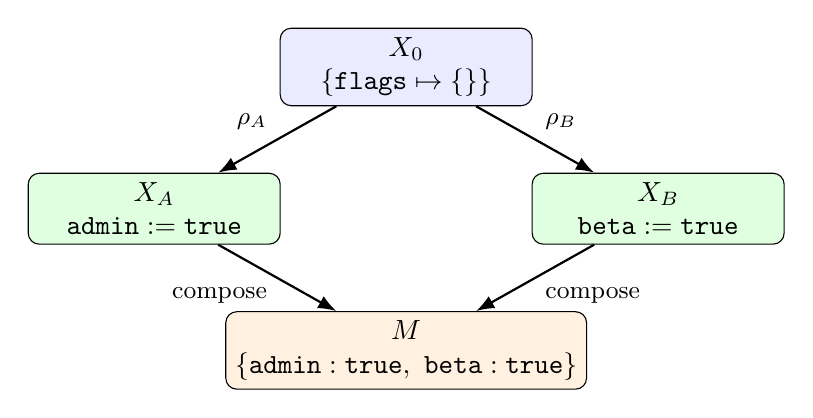
\begin{tikzpicture}[
  obj/.style={draw, rounded corners, minimum width=3.2cm, minimum height=0.9cm, align=center},
  base/.style={obj, fill=blue!8},
  brancha/.style={obj, fill=green!12},
  branchb/.style={obj, fill=green!12},
  merge/.style={obj, fill=orange!12},
  arr/.style={-Latex, thick}
]
\node[base] (x0) at (0,4.0) {$X_0$\\$\{\texttt{flags} \mapsto \{\}\}$};
\node[brancha] (xa) at (-3.2,2.2) {$X_A$\\$\texttt{admin} := \texttt{true}$};
\node[branchb] (xb) at (3.2,2.2) {$X_B$\\$\texttt{beta} := \texttt{true}$};
\node[merge] (m) at (0,0.4) {$M$\\$\{\texttt{admin}: \texttt{true},\ \texttt{beta}: \texttt{true}\}$};

\draw[arr] (x0) -- node[above left] {\small $\rho_A$} (xa);
\draw[arr] (x0) -- node[above right] {\small $\rho_B$} (xb);
\draw[arr] (xa) -- node[below left] {\small compose} (m);
\draw[arr] (xb) -- node[below right] {\small compose} (m);
\end{tikzpicture}
\caption{A text conflict below can correspond to independent rewrites upstairs.}
\end{figure}

\subsection{The merge upstairs}

The merge in the richer state space is trivial:
\[
\Merge(X_A,X_B)=
\{\texttt{flags} \mapsto \{\texttt{admin}:\texttt{true},\texttt{beta}:\texttt{true}\}\}.
\]

\subsection{Lowering back down}

Now we lower with a witness saying:
\begin{itemize}[leftmargin=2em]
\item serialize JSON canonically,
\item order keys lexicographically,
\item preserve booleans as JSON booleans.
\end{itemize}

Then the lowered public artifact is:

\begin{verbatim}
{"flags":{"admin":true,"beta":true}}
\end{verbatim}

\begin{observation}[What happened]
The conflict was real only in the lowered line-based view. In the richer
structural space, the edits were independent.
\end{observation}

\section{Example B: An AST / Source Example}

\subsection{The ordinary source surface}

Suppose the public artifact is a JavaScript module:

\begin{verbatim}
import { a } from "./lib";

export function run() {
  return a();
}
\end{verbatim}

Branch A adds a new helper import and uses it:

\begin{verbatim}
import { a, helper } from "./lib";

export function run() {
  helper();
  return a();
}
\end{verbatim}

Branch B reformats imports and changes ordering:

\begin{verbatim}
import {
  a
} from "./lib";

export function run() {
  return a();
}
\end{verbatim}

On text, these can collide around the same import block.

\subsection{The richer structured reading}

Upstairs, the relevant objects are:
\begin{itemize}[leftmargin=2em]
\item import specifier set for module \texttt{"./lib"},
\item function body statement list,
\item formatting policy as a lowering concern rather than branch semantics.
\end{itemize}

Branch A has two semantic rewrites:
\begin{enumerate}[leftmargin=2em]
\item add import specifier \texttt{helper},
\item prepend statement \texttt{helper();} to the function body.
\end{enumerate}

Branch B has no semantic change to the import set; it mostly changes lowering
policy of the same structure.

So a richer merge can:
\begin{itemize}[leftmargin=2em]
\item keep the import set \{\texttt{a}, \texttt{helper}\},
\item keep the function body with the helper call,
\item apply one canonical formatter while lowering.
\end{itemize}

\begin{observation}[Formatting is not semantics]
This example is useful because it shows a common category mistake: a source
control conflict often bundles semantic edits together with lowering-style
choices like ordering, wrapping, and pretty-printing.
\end{observation}

\section{Example C: A Genuine Semantic Conflict}

\subsection{The public artifact}

Suppose the public file says:

\begin{verbatim}
{"primaryColor":"blue"}
\end{verbatim}

Branch A changes it to:

\begin{verbatim}
{"primaryColor":"red"}
\end{verbatim}

Branch B changes it to:

\begin{verbatim}
{"primaryColor":"green"}
\end{verbatim}

\subsection{Lifted causal reading}

Upstairs, the semantic state is:
\[
X_0 = \{\texttt{primaryColor} \mapsto \texttt{blue}\}.
\]

Branch A applies:
\[
\rho_A : \texttt{primaryColor} := \texttt{red}.
\]

Branch B applies:
\[
\rho_B : \texttt{primaryColor} := \texttt{green}.
\]

The footprints overlap on the same invariant-bearing slot:
\[
\phi_A = \phi_B = \{\texttt{primaryColor}\}.
\]

There is no ordinary canonical state preserving both meanings at once if the
domain insists that \texttt{primaryColor} is singular.

\begin{figure}[h]
\centering
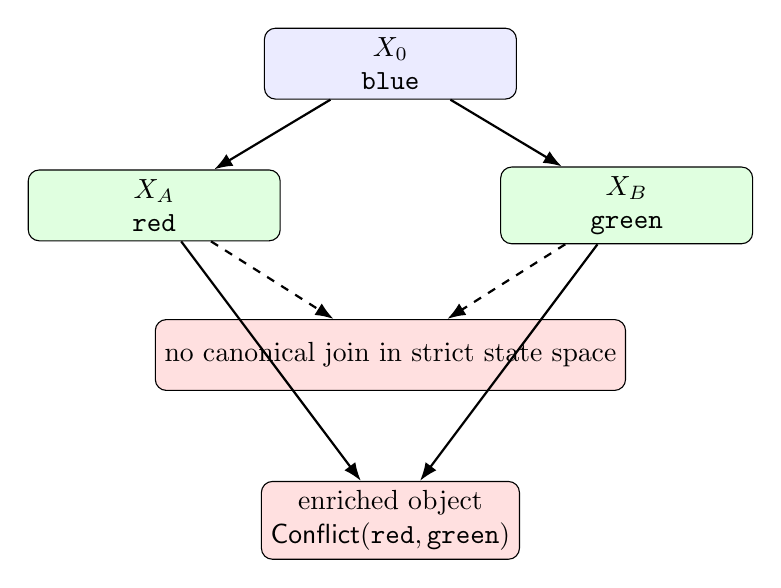
\begin{tikzpicture}[
  obj/.style={draw, rounded corners, minimum width=3.2cm, minimum height=0.9cm, align=center},
  base/.style={obj, fill=blue!8},
  branch/.style={obj, fill=green!12},
  conflict/.style={obj, fill=red!12},
  arr/.style={-Latex, thick}
]
\node[base] (x0) at (0,4.0) {$X_0$\\$\texttt{blue}$};
\node[branch] (xa) at (-3.0,2.2) {$X_A$\\$\texttt{red}$};
\node[branch] (xb) at (3.0,2.2) {$X_B$\\$\texttt{green}$};
\node[conflict] (c) at (0,0.3) {no canonical join in strict state space};
\node[conflict] (z) at (0,-1.8) {enriched object\\$\Conflict(\texttt{red},\texttt{green})$};

\draw[arr] (x0) -- (xa);
\draw[arr] (x0) -- (xb);
\draw[arr,dashed] (xa) -- (c);
\draw[arr,dashed] (xb) -- (c);
\draw[arr] (xa) -- (z);
\draw[arr] (xb) -- (z);
\end{tikzpicture}
\caption{A genuine semantic conflict does not disappear under lifting.}
\end{figure}

\subsection{What lifting still buys}

Lifting still matters here. It lets the system preserve:
\begin{itemize}[leftmargin=2em]
\item both intended values,
\item their causal provenance,
\item the obstruction witness,
\item later policy choices.
\end{itemize}

So instead of silently doing LWW or throwing an opaque text conflict, the
system can create:
\begin{itemize}[leftmargin=2em]
\item two strands,
\item a braid over the pair,
\item or an explicit conflict object.
\end{itemize}

\subsection{Lowering afterward}

Only after a policy decision may the system lower back to one public singleton
value.

That is not ``merge solved the conflict.'' It is:
\begin{quote}
merge preserved the conflict honestly, and lowering later consumed a policy
decision.
\end{quote}

\section{Example D: Governance Conflict}

Suppose a release-notes graph contains a public headline node. Branch A sets:
\[
\texttt{headline} := \texttt{"Fastest release yet"}
\]
while Branch B sets:
\[
\texttt{headline} := \texttt{"Stability first release"}
\]

Both edits are coherent. The public artifact still wants one headline. The
problem here is not that the state space lacks structure. The problem is that a
public projection wants one winner.

\begin{observation}[Policy is not the same as semantics]
This is why ``no merge conflicts ever'' is the wrong slogan. Some problems are
not failures of merge algebra. They are unresolved project policy.
\end{observation}

\section{A Full WARP Reading}

Using WARP nouns, the best interpretation is:
\begin{enumerate}[leftmargin=2em]
\item The shared base is a point on a \Worldline{}.
\item Each branch is a speculative \Strand{} carrying one causal lane.
\item A structured joint read may be expressed as a \Braid{}.
\item If the branches compose canonically, the result re-enters the canonical
  worldline directly.
\item If not, the braid or explicit conflict object preserves both until later
  collapse.
\end{enumerate}

\begin{figure}[h]
\centering
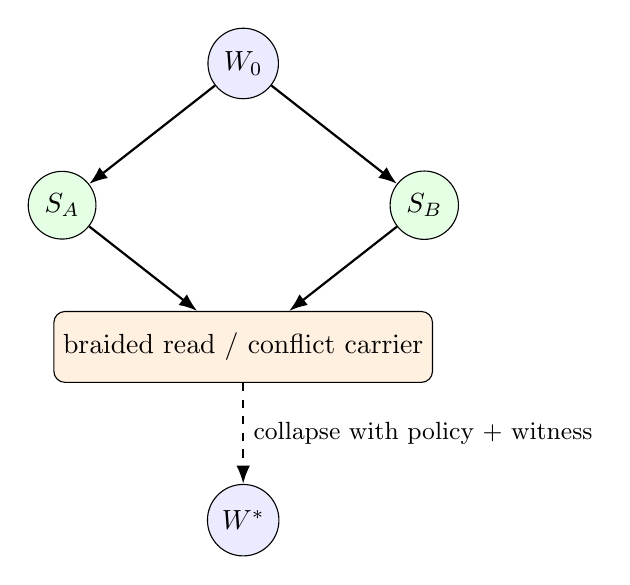
\begin{tikzpicture}[
  state/.style={draw, circle, minimum size=0.75cm, fill=blue!8},
  strand/.style={draw, circle, minimum size=0.75cm, fill=green!10},
  braid/.style={draw, rounded corners, minimum width=3cm, minimum height=0.9cm, fill=orange!12, align=center},
  arr/.style={-Latex, thick}
]
\node[state] (w0) at (0,4.2) {$W_0$};
\node[strand] (sa) at (-2.3,2.4) {$S_A$};
\node[strand] (sb) at (2.3,2.4) {$S_B$};
\node[braid] (b) at (0,0.6) {braided read / conflict carrier};
\node[state] (wc) at (0,-1.6) {$W^\ast$};

\draw[arr] (w0) -- (sa);
\draw[arr] (w0) -- (sb);
\draw[arr] (sa) -- (b);
\draw[arr] (sb) -- (b);
\draw[arr,dashed] (b) -- node[right] {\small collapse with policy + witness} (wc);
\end{tikzpicture}
\caption{WARP nouns let merge preserve alternatives instead of flattening them too early.}
\end{figure}

\section{Study Heuristic}

When you hit a merge problem, classify it with these questions:
\begin{enumerate}[leftmargin=2em]
\item Is the conflict only in the lowered view?
\item What are the real footprints upstairs?
\item Do the causal rewrites actually interfere?
\item If they interfere, is the problem semantic or governance?
\item If a richer merge exists, what witness do I need to lower it back?
\item If no canonical merge exists, what enriched object should preserve both
  sides honestly?
\end{enumerate}

\section{One-Sentence Summary}

The worked examples show the central rule: causal lifting can eliminate many
ordinary merge conflicts caused by lossy public surfaces, but when the branches
really disagree, the right move is not fake resolution but explicit preservation
of the obstruction, plus witness-backed lowering later.

\end{document}
